%%\documentclass[sn-nature]{sn-jnl}% Style for submissions to Nature Portfolio journals
%%\documentclass[sn-basic]{sn-jnl}% Basic Springer Nature Reference Style/Chemistry Reference Style
\documentclass[sn-mathphys,Numbered]{sn-jnl}
\usepackage{graphicx}%
\usepackage{multirow}%
\usepackage{amsmath,amssymb,amsfonts}%
\usepackage{amsthm}%
\usepackage{mathrsfs}%
\usepackage[title]{appendix}%
\usepackage{xcolor}%
\usepackage{textcomp}%
\usepackage{manyfoot}%
\usepackage{booktabs}%
\usepackage{algorithm}%
\usepackage{algorithmicx}%
\usepackage{algpseudocode}%
\usepackage{listings}%
\usepackage[normalem]{ulem}
\usepackage{comment}

% Make Orcid icon
\newcommand{\orcidicon}{
\includegraphics[width=0.32cm]{orcid.pdf}}
\newcommand{\orc}[1]{\href{https://orcid.org/#1}{\orcidicon}}

% Author Orcid ID: Define per author
\newcommand{\orcA}{0000-0001-8217-1484}
\newcommand{\orcB}{0000-0001-5038-8427}
\newcommand{\orcC}{0000-0001-5474-2649}
\newcommand{\orcD}{0000-0003-2704-6474}

% List of useful macros
\newcommand{\req}[1]{Eq.~(\ref{#1})}
\newcommand{\rf}[1]{Fig.~{\ref{#1}}}
\newcommand{\rt}[1]{Table~{\ref{#1}}}
\newcommand{\rsec}[1]{Sec.~{\ref{#1}}}
\newcommand*{\TeV}{\text{ TeV}}
\newcommand*{\GeV}{\text{ GeV}}
\newcommand*{\MeV}{\text{ MeV}}
\newcommand*{\keV}{\text{ keV}}
\newcommand*{\eV}{\text{ eV}}
\newcommand*{\meV}{\text{ meV}}
\DeclareMathOperator{\sgn}{sgn}

% Useful macros for annotation
\newcommand*{\xred}{\color{red}}
\newcommand*{\xblue}{\color{blue}}
\newcommand*{\xgreen}{\color{green}}
\newcommand*{\xmagenta}{\color{magenta}}
\newcommand{\rev}[1]{{\color{blue}#1}}
\newcommand*{\rcite}{{\xred (Citation?)}}

%\theoremstyle{thmstyleone}%
%\newtheorem{theorem}{Theorem}
%\newtheorem{proposition}[theorem]{Proposition}% 
%\theoremstyle{thmstyletwo}%
%\newtheorem{example}{Example}%
%\newtheorem{remark}{Remark}%
%\theoremstyle{thmstylethree}%
%\newtheorem{definition}{Definition}%

\raggedbottom
\begin{document}

%\title[Article Title]{Cold Ideal Fermi Gas}
\title[Article Title]{Zero and finite temperature  components of\newline Fermi quantum gas}

%%=============================================================%%
%% Prefix	-> \pfx{Dr}
%% GivenName	-> \fnm{Joergen W.}
%% Particle	-> \spfx{van der} -> surname prefix
%% FamilyName	-> \sur{Ploeg}
%% Suffix	-> \sfx{IV}
%% NatureName	-> \tanm{Poet Laureate} -> Title after name
%% Degrees	-> \dgr{MSc, PhD}
%% \author*[1,2]{\pfx{Dr} \fnm{Joergen W.} \spfx{van der} \sur{Ploeg} \sfx{IV} \tanm{Poet Laureate} 
%%                 \dgr{MSc, PhD}}\email{iauthor@gmail.com}
%%=============================================================%%
 
\author[1]{\hspace*{1.5cm}\fnm{Cheng Tao} \sur{Yang\orc{\orcB}}}
\author[1,2]{\fnm{Martin} \sur{Formanek\orc{\orcD}}}
\author[1]{\newline\fnm{Andrew} \sur{Steinmetz\orc{\orcC}}} 
\author[1]{\fnm{Jeremiah} \sur{Birrell\orc{\orcB}}}
\author[1]{\fnm{Johann} \sur{Rafelski\orc{\orcA}}}

%\email{iiiauthor@gmail.com}
%\equalcont{These authors contributed equally to this work.}

\affil[1]{\orgdiv{Department of Physics}, \orgname{The University of Arizona}, \city{\newline Tucson}, \state{Arizona}, \postcode{85721}, \country{USA}}

\affil[2]{\orgdiv{ELI Beamlines Facility}, \orgname{The Extreme Light Infrastructure ERIC}, \orgaddress{ \postcode{\newline 252 41}  \city{Doln\'{i} B\v{r}e\v{z}any}, \country{Czech Republic}}}

\abstract{We present a novel mathematical tool allowing to separate the zero and finite temperature phenomena in ideal Fermi gases. To achieve this  we decompose the Fermi distribution into three components. We prove that the singular (step) functions properly add up to the finite temperature smooth Fermi shape. As an example we consider briefly a semi relativistic-electron density where with high chemical potential ($\mu>m$) at low temperature $T<<m$.}

% ANDREW's note: We present a novel mathematical tool allowing the separation of the finite and zero temperature phenomena in fermi gassses. To achieve this, we provide a novel form of the Fermi distribution 

\date{January 2024, To be published in International Journal of Theoretical Physics}
\keywords{Fermi distribution, Low temperature}

%%\pacs[JEL Classification]{D8, H51}
%%\pacs[MSC Classification]{35A01, 65L10, 65L12, 65L20, 65L70}

\maketitle

%%%%%%%%%%%%%%%%%%%%%%%%%%%%%%%%%%%%%%%
\section{Introduction}
\label{sec1}
%%%%%%%%%%%%%%%%%%%%%%%%%%%%%%%%%%%%%%%

% Andrew's note (2/26/2024): Can the 1st derivative delta function problem present in other mathematical examples of derivatives of distributions? If so, then this clarifies the issue and separates it entirely from the complexity of the FD distribution. Suggested mathematical example to try: f(x) = FD(x) - Heaviside(x). Hmm...

% Second solution idea: Redo the derivative derivation however treating all singular functions as couched within an integration. E.g. no naked distributions! Do then physical measurable quantities suffer from this inconsistancy? I suspect not. Therefore there is no problem.

The  zero temperature limit of Fermi-Dirac (FD) distribution involves a transition from a smooth functional form to a singular Heavyside step function. Such singular limit  $
T\to 0$ therefore cannot be analytical.  For this reason a study of finite temperature effects in dense  low temperature  FD quantum gasses poses a mathematical challenge and can miss key physical features.  To remedy this situation we introduce here a novel reformulation which allows exact separation of the finite temperature behavior from the singular zero temperature limit. This means that we will be replacing the smooth FD distribution by the sum of three singular functions
$$
\boxed{\frac{1}{e^{x} +1}=\Theta(-x)+\frac{1}{2}e^{-|x|}\left[\sgn(x)+\tanh(x/2)\right]}
$$
one being the $T=0$ limit,  the other two describing the finite temperature residual. In the following we illuminate the advantages offered by this decomposition.  


The most interesting physics of FD gasses occurs at finite temperatures~\cite{Elze:1980er} which necessitates a mathematical tool which captures the finite temperature behavior of the FD distribution. We provide a novel form of FD distribution that manifestly separates the zero and finite temperature contributions so that the finite temperature correction can be studied on its own. We also tackle the case of the semi-relativistic electron gas to demonstrate the usefulness of this new method. Other use cases would be for compact astrophysical systems (white dwarfs, neutron stars, quark stars)~\cite{Kaspi:2017fwg,Ferrer:2019xlr,Ferrer:2023pgq}, Early Universe phenomenology~\cite{Rafelski:2021aey,Rafelski:2023emw,Grayson:2023flr,Steinmetz:2023nsc}, quark-gluon plasmas (QGP)~\cite{Letessier:2002ony,Rafelski:2020ajx,Yang:2021bko}, and in any situation when finite temperature Fermi effects are important.

%Before we introduce the novel form in \rsec{NewFermi}, we will briefly recall the standard picture of the FD distribution. 

The illustration of the problem is presented in \rf{Electron_001}: In the zero temperature limit $T\to0$, the FD distribution reduces to a step function where a state $E_{i}$ is either filled or empty. For given chemical potential $\widetilde\mu(T)$, we have
\begin{align}
\label{f_old}
f_\mathrm{FD}[E_{i},\widetilde\mu(T),T]=\left[\exp\left(\frac{E_{i}-\widetilde\mu}{T}\right)+1\right]^{-1}\,,\quad
\lim_{T\to0}f_\mathrm{FD}=\left\{
\begin{array}{c}
1,\quad\mathrm{for}\quad{E_{i}}<\widetilde\mu\\
0,\quad\mathrm{for}\quad{E_{i}}>\widetilde\mu
\end{array}
\right.\,.
\end{align}
The energy of the last filled state is called the Fermi energy and is denoted by $E_F$. The Fermi energy is also the value of the chemical potential at zero temperature $T=0$, \emph{i.e.} $E_F\equiv\widetilde\mu(T = 0)$.
%%%%%%%%%%%%%%%%%%%%%%%%%%%%%%%%%%%%%%%
\begin{figure}[ht]
\centering
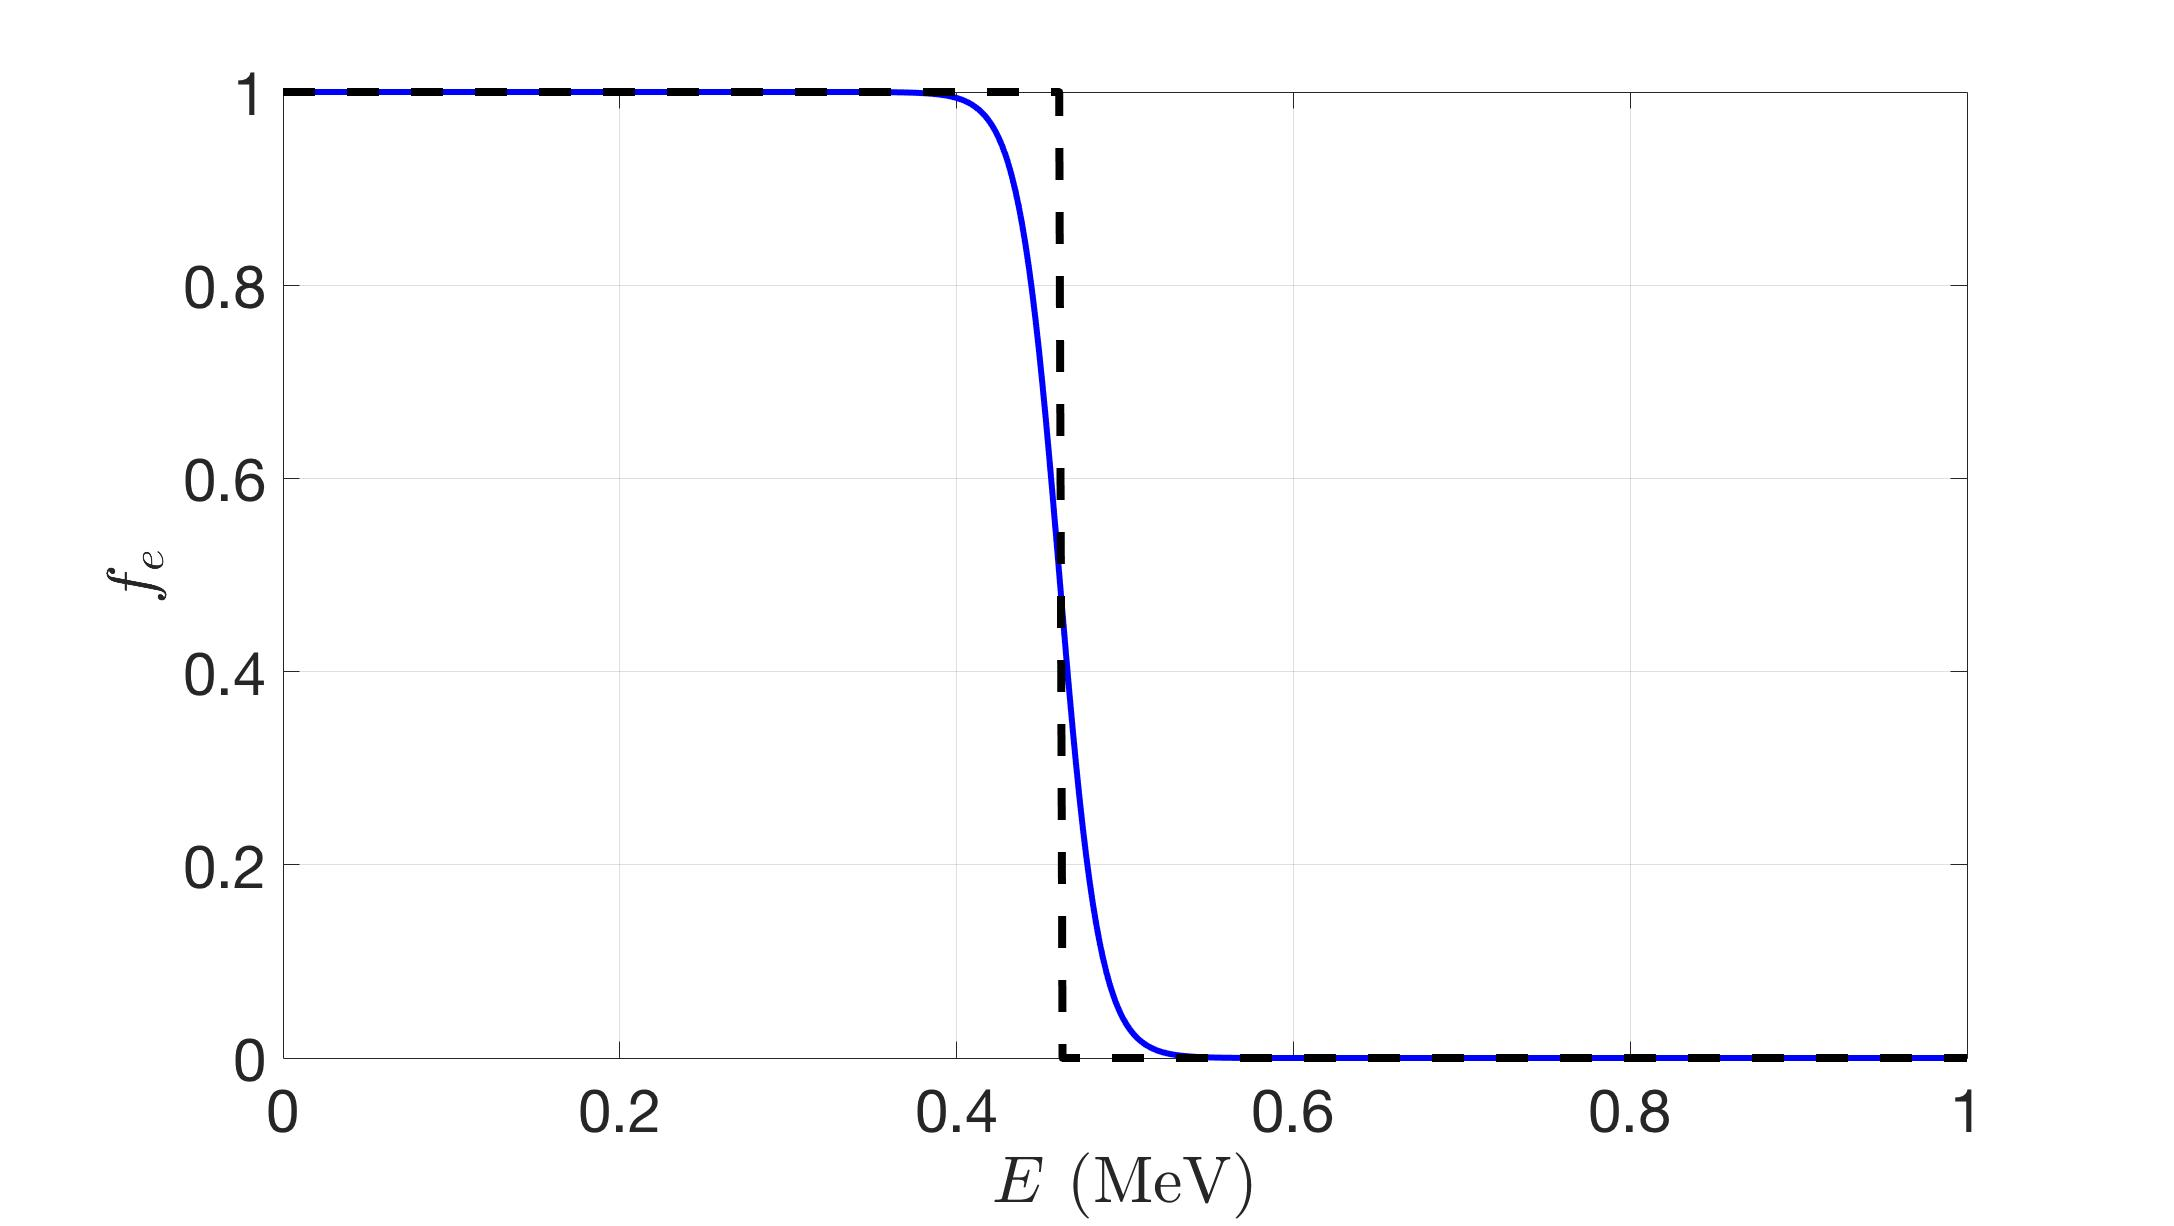
\includegraphics[width=0.9\textwidth]{./plot/Electron_distribution001}
\caption{The FD distribution is plotted (solid blue line) as a function of energy with parameters $T=0.012\MeV$ and $\widetilde\mu=0.461\MeV$. The zero temperature distribution is plotted as the dashed black line.}
\label{Electron_001}
\end{figure}
%%%%%%%%%%%%%%%%%%%%%%%%%%%%%%%%%%%%%%%

In \rf{Electron_001} the solid line shows Fermi distribution as a function of energy for temperature $T=0.012\MeV$, chemical potential $\widetilde\mu=0.461\MeV$, and electron mass $m=0.511\MeV$. Dashed line is the corresponding $T=0$ limit.  This demonstrates the textbook behavior that for finite temperature $T > 0$, even states above the chemical potential $\widetilde\mu$ can be occupied at the expense of states below $\widetilde\mu$. As the temperature increases, the distribution becomes broader as a wide range of states become thermally populated.

Our objective is to describe the difference between these two distributions in a format allowing to evaluate and study in semi-analytical way the finite temperature effects occuring near to the Fermi surface.

%%%%%%%%%%%%%%%%%%%%%%%%%%%%%%%%%%%%%%%
\section{Zero and finite temperature Fermi-Dirac distributions}
\label{NewFermi}
%%%%%%%%%%%%%%%%%%%%%%%%%%%%%%%%%%%%%%%
\subsection{A novel form of Fermi-Dirac distribution}
\label{Novel}
%%%%%%%%%%%%%%%%%%%%%%%%%%%%%%%%%%%%%%%
Our interest and motivations in studying the Fermi-Dirac distribution was to perform cosmological computations involving both high and low temperature physics. In doing so, we have identified the following novel way to write FD distribution as three terms which separates out the zero temperature portion from the finite temperature contributions as 
\begin{align}
\label{NFF1}
\begin{split}
f_\mathrm{FD}(x)
&=\frac{1}{e^{x}+1}\,,\quad
x\equiv\frac{E-\widetilde\mu}{T}\,,\\
\frac{1}{e^{x} +1}&=\Theta(-x)+\frac{1}{2}e^{-|x|}\left[\sgn(x)+\tanh(x/2)\right]
\,,
\end{split}
\end{align}
\begin{align}
\label{NFF2}
\Theta(x)=\left\{
\begin{array}{r}
1,\quad\mathrm{for}\quad{x}>0\\
%1/2,\quad\mathrm{for}\quad{x}=0\\
0,\quad\mathrm{for}\quad{x}<0
\end{array}\right.\,,\qquad
\sgn(x)=\left\{
\begin{array}{r}
+1,\quad\mathrm{for}\quad{x}>0\\
%0,\quad\mathrm{for}\quad{x}=0\\
-1,\quad\mathrm{for}\quad{x}<0\\
\end{array}\right.\,,
\end{align}
where $\Theta(x)$ is the Heaviside step function and $\sgn(x)$ is the sign function {\xgreen whose values at $x=0$ are convention-dependent and do not affect our results}. The first term $\Theta(-x)$ in \req{NFF1} represents the zero temperature portion of the FD distribution while the finite temperature terms are weighted by a decaying exponential function. The immediate benefit of this form is that numerical evaluations will naturally center around the Fermi surface of the system with finite temperature contributions exponentially weighted.

We note that \req{NFF1} comprises of distributions rather than analytical functions~\cite{Arfken:2011abc}. On first sight, it is difficult to see that these cancel to create the analytical FD function seen in \req{f_old}. In the following section, we will show that both sides are truly equivalent.

%%%%%%%%%%%%%%%%%%%%%%%%%%%%%%%%%%%%%%%
\subsection{Mathematical proof}
\label{Proof}
%%%%%%%%%%%%%%%%%%%%%%%%%%%%%%%%%%%%%%%
To show the equivalency between the two distinct forms of the FD, we look at the three relevant regions of $x>0$, the origin $x=0$, and $x<0$. For $x>0$, \req{NFF1} evaluates as
\begin{equation}\label{eq:xpos}
    f_\mathrm{FD}(x>0) = 0 + \frac{1}{2}e^{-x}[1+\tanh(x/2)] = (e^x + 1)^{-1}\,.
\end{equation}
This can be seen by using the hyperbolic formula $\tanh(x/2)=(e^x-1)/(e^x+1)$. In a similar manner, the $x<0$ region evaluates as
\begin{equation}\label{eq:xneg}
    f_\mathrm{FD}(x<0) = 1 + \frac{1}{2}e^{x}[-1 + \tanh(x/2)] = (e^x + 1)^{-1}\,.
\end{equation}

As our expression is written in terms of distributions rather than analytic functions, {\xgreen we need to compare with the original prescription in the sense of integration over a infinitely-differentiable compactly-supported test function $\phi(x)$
\begin{equation}
    \langle f_\text{FD}, \phi \rangle \equiv \int_{-\infty}^\infty f_\text{FD}(x) \phi(x) dx  = \langle (e^x + 1 )^{-1}, \phi\rangle\,.
\end{equation}
The last equality holds since the integration can be broken into integrals over $(-\infty,0)$ and $(0,\infty)$ and using Eqs.~(\ref{eq:xpos},\ref{eq:xneg}). The exact behavior of functions $\Theta(x)$ and $\text{sgn}(x)$ at $x=0$ depends on a convention and it is not necessary for showing equality in terms of distributions since the point $x=0$ represents a set of measure zero with respect to integration.}

\begin{comment}
special care should be taken in evaluation of the origin. It can be shown that the left $x=0^{-}$ and right $x=0^{+}$ limits are equal via
\begin{align}
    \lim_{x\rightarrow 0^+} f_\mathrm{FD}(x) &= 0 + \frac{1}{2}(1 + 0) = \frac{1}{2}\,,\\
    \lim_{x\rightarrow 0^-} f_\mathrm{FD}(x) &= 1 + \frac{1}{2}(-1 + 0) = \frac{1}{2}\,,
\end{align}
which means that the limit of our expression at the origin $x=0$ exists and is equal to the value of the function in \req{f_old} at $x = 0$. With the definitions of the step function $\Theta(x)$ and sign function $\sgn(x)$ in \req{NFF2}, the limits for $x\rightarrow0^{\pm}$ are equal to the value of our function at the origin. Therefore, for all real $x\in\mathbb{R}$, our expression matches the original FD distribution \req{f_old}.
\end{comment}

\begin{comment}
Lastly, we check that the properties of the first derivative of \req{NFF1} are in agreement with the usual FD distribution. We write the first derivative of the singular distributions as 
\begin{align}
\label{NFF1b}
\frac{d}{dx}\Theta(-x)&=-\delta(x)\,,\qquad 
\frac{d}{dE}\Theta(-x)=-\frac{1}{T}\delta(x)\,,\\
\frac{d}{dx}\sgn(x)&=2\delta(x)\,,\,\,\quad 
\frac{d}{dE}\sgn(x)=\frac{2}{T}\delta(x)\,,
\end{align}
both without and with units and where $\delta(x)$ is the Dirac $\delta$-function. \rev{The first derivative of the original FD distribution is
\begin{equation}\label{eq:ffdder}
    \frac{d}{dE} f_{FD}(x) = \frac{1}{T} \frac{-1}{4\cosh^2 \frac{x}{2}}
\end{equation}
which goes in the $T \rightarrow 0^+$ limit to delta function (DOES IT REALLY? NORMALLY $\delta$ is limit of 1/cosh). Using
\begin{equation}
    \frac{d|x|}{dE} = \frac{d\text{sgn}(x)x}{dE} = \frac{1}{T}\text{sgn}(x) + \frac{2}{T}x\delta(x)
\end{equation}
we can evaluate the derivative of the novel form as 
\begin{equation}
    \begin{split}
    T \frac{d}{dE}f_N(x) &= -\delta(x) - \frac{1}{2}e^{-|x|}[\text{sgn}(x) + 2x\delta(x)]\text{sgn}(x) + e^{-|x|}\delta(x)\\
    &- \frac{1}{2}e^{-|x|}[\text{sgn}(x) + 2 x \delta(x)]\tanh\frac{x}{2} + \frac{1}{4}\frac{e^{-|x|}}{\cosh^2\frac{x}{2}}
    \end{split}
\end{equation}
It is quite straightforward to show that for $x > 0$ or $x<0$ this expression matches Eq. (\ref{eq:ffdder}) as it should because outside $x=0$ we don't expect any issues. For $x\neq 0$ we have
\begin{equation}
    \begin{split}
    \left. T \frac{d}{dE}f_N(x)\right|_{x\neq 0} &= -\frac{1}{2}e^{-|x|} - \frac{1}{2}e^{-|x|}\tanh\frac{|x|}{2} + \frac{1}{4}\frac{e^{-|x|}}{\cosh^2\frac{|x|}{2}}\\
    &= \frac{-e^{-|x|}\left(2\cosh^2\frac{|x|}{2}+2\sinh\frac{|x|}{2}\cosh\frac{|x|}{2}-1\right)}{4\cosh^2\frac{|x|}{2}}
    \end{split}
\end{equation}
Now we re-write $1 = \cosh^2|x|/2 - \sinh^2|x|/2$ and use the twice angle formulas $\cosh^2|x|/2 + \sinh^2|x|/2 = \cosh|x|$ and $2\sinh |x|/2 \cosh|x|/2 = \sinh|x|$
\begin{equation}
    \left. T \frac{d}{dE}f_N(x)\right|_{x\neq 0} = -\frac{e^{-|x|}\left(\cosh|x|+\sinh|x|\right)}{4\cosh^2\frac{|x|}{2}} = \frac{-1}{4\cosh^2\frac{|x|}{2}}
\end{equation}
since $\cosh|x| + \sinh|x| = e^{|x|}$. However, the behavior of the first derivative at $x = 0$ is strange and does not match \req{eq:ffdder}. The question is if we care about the single point $x=0$, since if integrated over a whole set of functions, this should not change the behavior of the distribution corresponding to the first derivative. 
}


\rev{NOT TRUE:} These cancel in \req{NFF1} at $x=0$ exactly as required since the derivative of the FD distribution written in \req{f_old} lacks a $\delta$-function. This encourages us to believe that all of singular expressions cancel leaving it fully analytic. This completes our demonstration of the validity of \req{NFF1}.

{\bf JB: There are some details missing regarding exactly what you are finding to be strange about $x=0$ but here are some general comments as to what I believe is the issue. First, you using the product rule which can fail for the product of nonsmooth distributions if things are singular enough.  In your problem, the situation isn't that bad: the product rule holds in the sense of distributions but not pointwise, and it seems like you are trying to make pointwise comparisons.  However, as soon as you start taking derivatives in the sense of distributions then pointwise comparisons are not necessarily valid: equality now only has meaning in terms of integrals against test functions.  If you give more details regarding the issue you are encountering then maybe I comment more specifically on your calculation.  However, when I do the calculation, I get the expected equality in the sense of distributions:}\\
First
\begin{align}
    \frac{d}{dx} e^{-|x|}=-\text{sgn}(x)e^{-|x|}
\end{align}
Next:
\begin{align}
    \frac{d}{dx}(e^{-|x|}\text{sgn}(x))=2\delta(x)-e^{-|x|}
\end{align}
For this term one should be careful because it is the product of two non-smooth functions and so the product rule could fail.  However, nothing too crazy happens here, though one should note that the result only meaningful in the sense of distributions.  To carefully check this result, let $\phi(x)$ be a smooth compactly supported test function and compute
\begin{align}
    &\langle  \frac{d}{dx}(e^{-|x|}sgn(x)),\phi\rangle\\
    =&-\int_{\infty}^\infty e^{-|x|}sgn(x)\phi^\prime(x) dx\\
    =&2\phi(0)-\int_{-\infty}^\infty e^{-|x|}\phi(x) dx\\
    =&\langle 2\delta(x)-e^{-|x|},\phi\rangle
\end{align}
To get the from the second line to the third line, break the integral into integrals over $(-\infty,0)$ and $(0,\infty)$ and integrate each term by parts.

In the term $e^{-|x|}\tanh(x/2)$, one of the terms is smooth so one can use the product rule without worry.  Therefore we can put these pieces together to get
\begin{align}
    &\frac{d}{dx} f_N(x)\\
    =&-\delta(x)+\frac{1}{2}(2\delta(x)-e^{-|x|})+\frac{1}{2}(-\text{sgn}(x)e^{-|x|})\tanh(x/2)+\frac{1}{4}e^{-|x|}\frac{1}{\cosh^2(x/2)}\\
    =&-\frac{1}{2}e^{-|x|}+\frac{1}{2}(-\text{sgn}(x)e^{-|x|})\tanh(x/2)+\frac{1}{4}e^{-|x|}\frac{1}{\cosh^2(x/2)}\\
    =&\frac{-1}{4\cosh^2(x/2)}
\end{align}
{\bf
Note that the equality in the last line holds pointwise in terms of functions, but that is not strictly necessary to have equality in terms of distributions: if either side differed on a set of measure zero (e.g., if they differed at $0$) then equality in the sense of distributions would still hold, and since we took derivatives in the sense of distributions that is the most one could reasonably expect.  It is certainly possible to do the above calculation in a different way and get an answer that differs at $0$ but is equal everywhere else, and that would still prove equality in the sense of distributions; I think you are running into the latter situation in your caclucation, but without more details I can't be sure.
}
\end{comment}

%%%%%%%%%%%%%%%%%%%%%%%%%%%%%%%%%%%%%%%
\subsection{Decomposition of zero and finite temperature contribution}
\label{Numerical}
%%%%%%%%%%%%%%%%%%%%%%%%%%%%%%%%%%%%%%%
%%%%%%%%%%%%%%%%%%%%%%%%%%%%%%%%%%%%%%%

%{\xmagenta ANDREW: I recommend we stick with the dimensionless variable ``$x$'' for all calculations and discussions up to the physical example. This enhances the mathematical clarity and simply makes the expressions more simple to read. I did this for Eq. 11, but wanted your approval before continuing my edits. Additionally, the expression $f_{T=0}(x)$ doesn't make sense as $T$ is clearly nonzero in $x(E,\widetilde\mu,T)$. I suggest we abandon this notation and simply call it the step function $\Theta(x)$ and we are already doing earlier. There is also a conflict where Eq. 12 and Eq. 13 are defined using the same notation. Is this an error? Please look at this Cheng Tao.} 
To illustrate the separation of the zero and finite temperature contributions to the FD distribution, it is convenient to rewrite Eq.~(\ref{NFF1}) in the following form
\begin{align}\label{Eq_form}
&f_\mathrm{FD}(x)=\Theta(-x)+f_\mathrm{T\neq0}(x)+\tilde f_\mathrm{T\neq0}(x)
\end{align}
where the temperature functions are defined as
\begin{align}
&f_\mathrm{T\neq0}=\frac{1}{2}e^{ -|x| }\mathrm{sgn}\left(x\right),\qquad
\tilde f_\mathrm{T\neq0}=\frac{1}{2}e^{ - |x| }\tanh\left(\frac{x}{2}\right),\qquad x=\frac{E-\tilde\mu}{T}
%&f_\mathrm{T\neq0}=\frac{1}{2}e^{ - |E-\widetilde\mu|/T }\mathrm{sgn}\left(\frac{E-\widetilde\mu}{T}\right),\qquad
%\tilde f_\mathrm{T\neq0}=\frac{1}{2}e^{ - |E-\widetilde\mu|/T }\tanh\left(\frac{E-\widetilde\mu}{2T}\right)
\end{align}
In Fig.~\ref{Fermi_Component} we plot the exact Fermi distribution (black line $f$), the zero (purple lines, $\Theta(-x)$) and finite temperature components of the Fermi distribution as a function of energy choosing in this example the chemical potential $\widetilde\mu=0.461\MeV$ at temperature $T=0.02\MeV$ and at $T=0.2\MeV$.

%%%%%%%%%%%%%%%%%%%%%%%%%%%%%%%%%%%%%%%
\begin{figure}[ht]
\centering
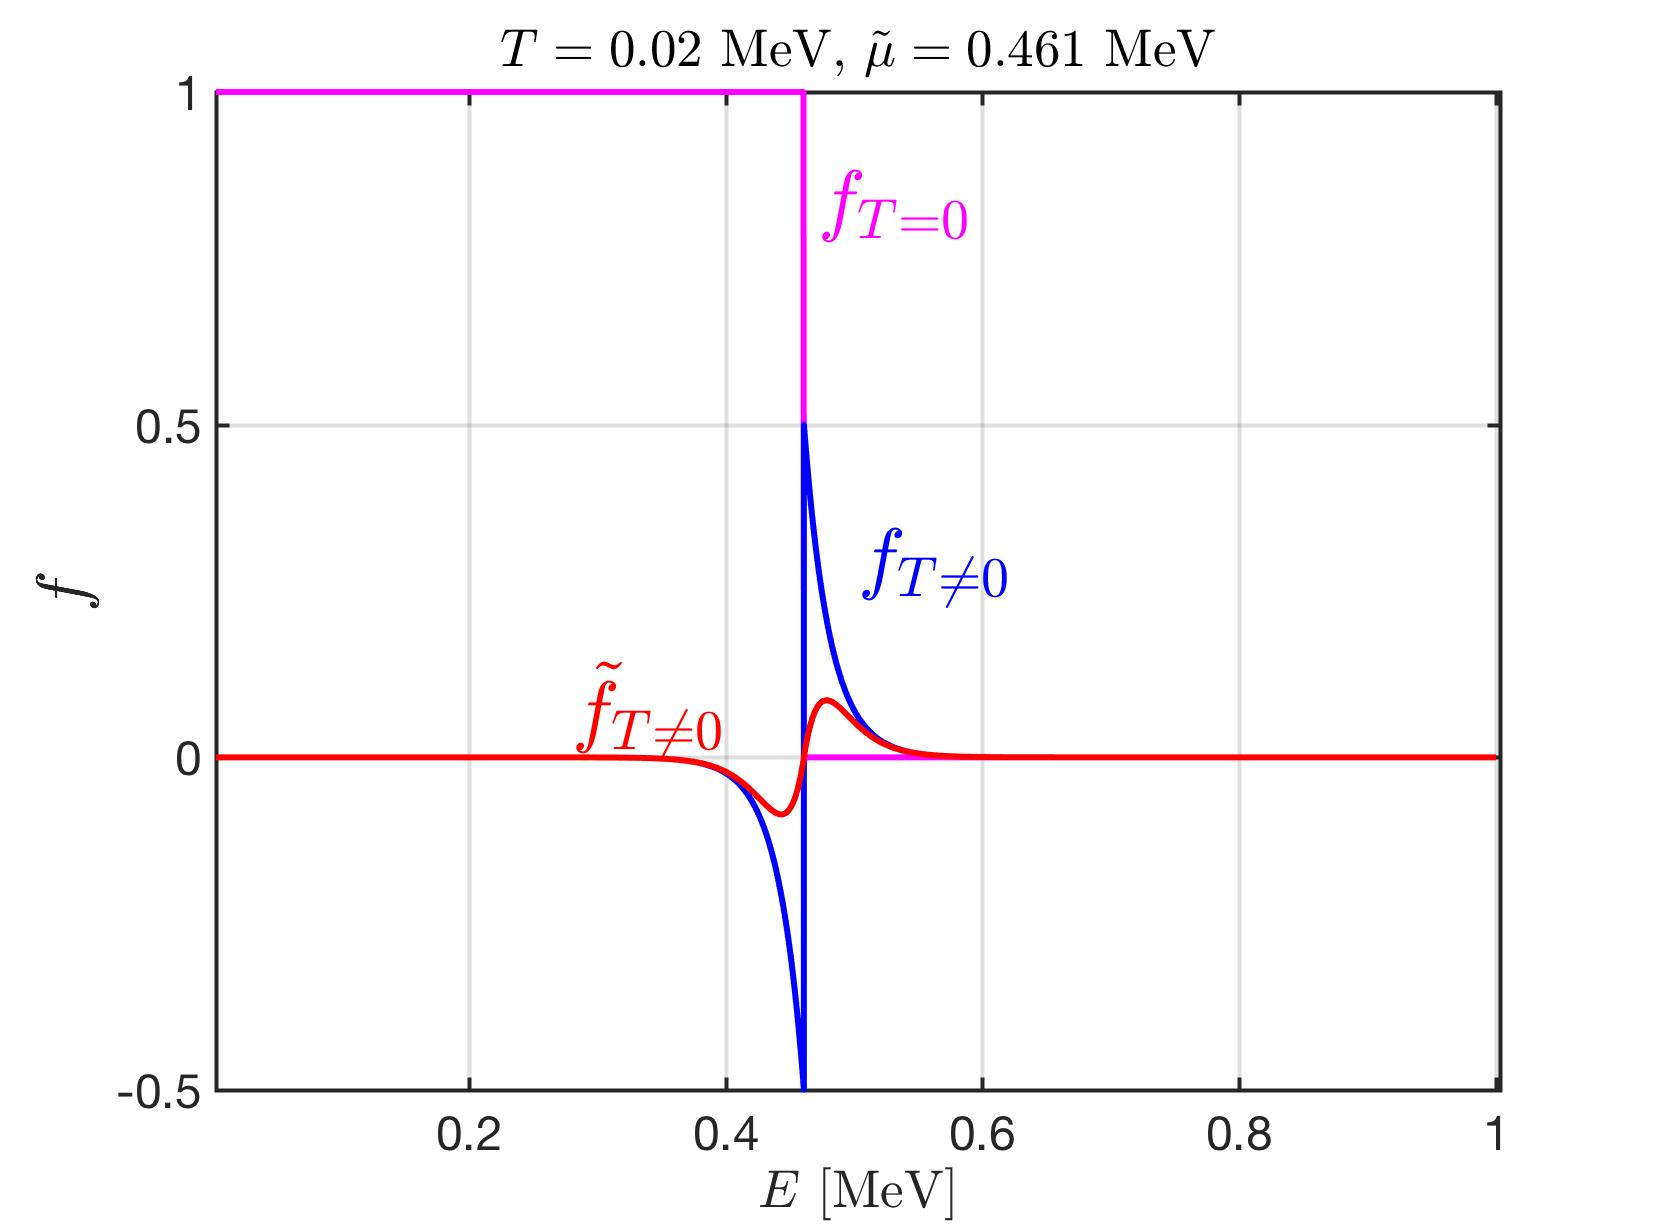
\includegraphics[width=0.5\textwidth]{./plot/FermiZeorFiniteTemperature}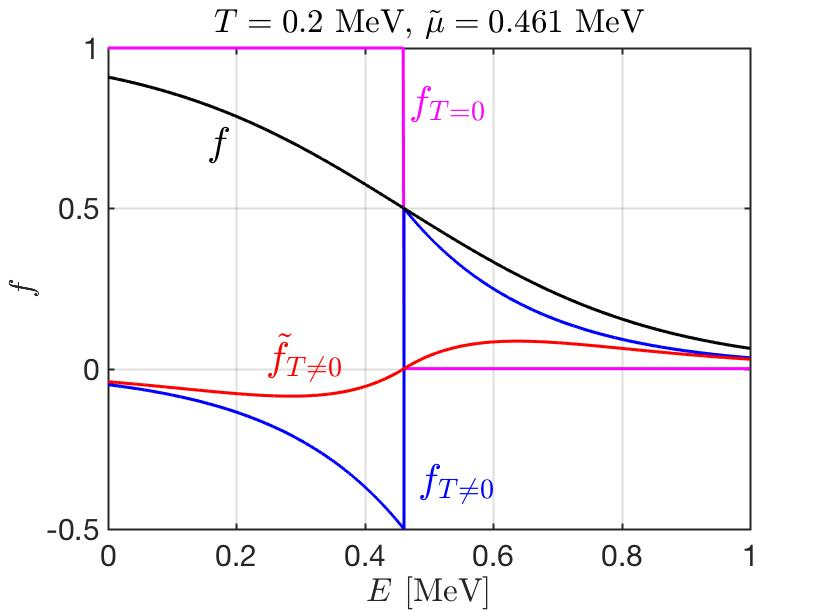
\includegraphics[width=0.5\textwidth]{./plot/FermiZeroFiniteTemperature002}
\caption{%\rev{Here I would add the full fermi distribution - to see how it is decomposed to zero temperature and finite temperature terms.}
The zero and finite temperature components of the decomposition here considered for Fermi distribution as a function of energy with chemical potential $\widetilde\mu=0.461\MeV$ at temperature $T=0.02\MeV$ and $T=0.2\MeV$. The black line represents the exact Fermi distribution. The purple line represents the zero temperature component $f_{\mathrm{T}=0}$, and blue and red lines represent the finite temperature components $f_\mathrm{T\neq0}$ and $\tilde f_\mathrm{T\neq0}$ respectively. }
\label{Fermi_Component}
\end{figure}
%%%%%%%%%%%%%%%%%%%%%%%%%%%%%%%%%%%%%%%

The Fig.~(\ref{Fermi_Component}) shows that \rev{the contributions of the two finite temperature components $f_\mathrm{T\neq0}$ and $\tilde f_\mathrm{T\neq0}$ exponentially decay with the distance from the Fermi surface $E=\tilde{\mu}$. Moreover, the splitting was chosen in such a way that the discontinuous distribution part is fully contained in $f_\mathrm{T\neq 0}$ and $\tilde{f}_\mathrm{T\neq 0}$ is a remaining continuous function of temperature $T$.}  Both finite temperature contributions always have the same sign \rev{and lower the distribution for $E < \tilde{\mu}$ and increase it for $E > \tilde{\mu}$}.

In contrast to the brute force approach for eliminating the $T=0$ limit from the low-temperature Fermi distribution, our analytic form of distribution offers a more numerically advantageous method for separating the finite temperature components. This is advantage arise from the behavior of: 1.) both finite temperature contributions $f_\mathrm{T\neq0}$ and $\tilde f_\mathrm{T\neq0}$ always have the same sign 2.) the exponential factor for finite temperature components provide the naturally exponentially suppresses for the large energy. In this scenario, it reduces the numerical noise when evaluate the numerical integral beyond the zero temperature approximation. Furthermore, our novel form for Fermi distribution also provide us the tool to analytically investigate the finite temperature contributions by expanding the function around the Fermi-energy surface, which is useful for addressing physics for the finite temperature approximation.

\subsection{Numerical illustration}
To illustrate the advantage of our novel form of distribution can be used to address the integrals common in statistical physics especially when temperature $T\to0$, we examine the thermal average of any given function $G(p)$ . This thermal average physical quantity, denoted as $\langle G\rangle_T$, is determined by integrating over the D-dimensional phase space 
\begin{align}
\langle G\rangle_T&\equiv\int^{\infty}_{0}\!\!\frac{d^Dp}{(2\pi)^D}\,G(p)\,f_{FD}(p)=\frac{1}{(2\pi)^D}\frac{2\pi^{D/2}}{\Gamma(D/2)}\int^{\infty}_{0}\!\!dp\,p^{D-1}\,G(p)\,f_{FD}(p).
\end{align}
By Substituting our novel form of FD distribution, the physical quantity $\langle G\rangle_T$ can be expressed as the sum of three distinct components:
\begin{align}
\langle G\rangle_T=\langle G\rangle_{\Theta}+\langle G\rangle_{\delta T}+\langle G\rangle_{\delta \tilde T},
\end{align}
 where the functions $\langle G\rangle_{\Theta}$, $\langle G\rangle_{\delta T}$ and $\langle G\rangle_{\delta \tilde T}$ are defined as
\begin{align}
&\langle G\rangle_{\Theta}=\frac{1}{(2\pi)^D}\frac{2\pi^{D/2}}{\Gamma(D/2)}\int^{\infty}_{0}\!\!dp\,p^{D-1}G(p)\Theta\left(\frac{-E+\tilde\mu}{T}\right),\qquad E=\sqrt{p^2+m^2},\\
\label{G_deltaT}
&\langle G\rangle_{\delta T}=\frac{1}{(2\pi)^D}\frac{2\pi^{D/2}}{\Gamma(D/2)}\int^{\infty}_{0}\!\!dp\,p^{D-1}\,G(p)\,f_\mathrm{T\neq0}(p),\\
\label{G_deltaT2}
&\langle G\rangle_{\delta \tilde T}=\frac{1}{(2\pi)^D}\frac{2\pi^{D/2}}{\Gamma(D/2)}\int^{\infty}_{0}\!\!dp\,p^{D-1}\,G(p)\,\tilde f_\mathrm{T\neq0}(p).
\end{align}

To simplify the integral we can utilize the Laguerre polynomials $L_n(y)$ as a orthogonal basis to expand the  functions. These polynomials satisfies the orthogonality condition as follows
\begin{align}
L_n(p)=\frac{e^p}{n!}\frac{d^n}{dp^n}\left(p^ne^{-p}\right),\qquad\int_0^\infty\!\!dpL_n(p)L_m(p)e^{-p}=\delta_{nm}
\end{align}
In this scenario, the functions $p^{D-1}G(p)$, $f_\mathrm{T\neq0}(p)$, and $\tilde f_\mathrm{T\neq0}(p)$ involved in the integrals can be expressed in terms of Laguerre polynomials as
\begin{align}
&p^{D-1}G(p)=\sum_{n=0}^\infty k_nL_n(p),\qquad\quad k_n=\int_0^\infty\!\!dp\,p^{D-1}G(p)L_n(p)e^{-p}\\
&f_\mathrm{T\neq0}(p)=\sum_{m=0}^\infty a_m e^{-p}L_m(p),\qquad a_m=\int_0^\infty\!\!dp f_\mathrm{T\neq0}(p)L_m(p)\\
&\tilde f_\mathrm{T\neq0}(p)=\sum_{m=0}^\infty b_m e^{-p}L_m(p),\qquad b_m=\int_0^\infty\!\!dp \tilde f_\mathrm{T\neq0}(p)L_m(p)
\end{align}
where $k_n$, $a_m$ and $b_m$ represent the expansion coefficients. By substituting the polynomial expansion into Eq.~(\ref{G_deltaT}) and Eq.~(\ref{G_deltaT2}) for the finite temperature contribution, the integral of $\langle G\rangle_{\delta T}+\langle G\rangle_{\delta \tilde T}$ becomes
\begin{align}
\langle G\rangle_{\delta T}+\langle G\rangle_{\delta \tilde T}&=\frac{1}{(2\pi)^D}\frac{2\pi^{D/2}}{\Gamma(D/2)}\int^{\infty}_{0}\!\!dp\,\left[\sum_{n=0}^\infty k_nL_n(p)\right]\left[\sum_{m=0}^\infty \left(a_m+b_m\right) e^{-p}L_m(p)\right]\notag\\
&=\frac{1}{(2\pi)^D}\frac{2\pi^{D/2}}{\Gamma(D/2)}\sum_{n,m=0}^\infty k_n(a_m+b_m)\left[\int_0^\infty\!\!dp e^{-p}L_n(p)L_m(p)\right]\notag\\
&=\frac{1}{(2\pi)^D}\frac{2\pi^{D/2}}{\Gamma(D/2)}\sum^\infty_{n=0}k_n(a_n+b_n).\label{Sum000}
\end{align}
We use the orthogonal property of Laguerre polynomial to express the integral as an infinite sum of coefficients $a_n$, $b_n$, and $k_n$. This method simplifies the evaluation of the finite temperature integral and provides a powerful too for investigating the finite temperature behavior under different temperature conditions.

% Andrew's note: CHECK EQ. 23 for accuracy. The othogonality implementation is suspect to me.

To demonstrate the equivalence between our novel distribution and the Fermi-Dirac distribution for any thermal average physical quantity, we examine the semi-relativistic electron number density with a chemical potential $\mu>m$ as an example.  Given the exact Fermi-Dirac distribution, the number density  in $3$-dimension phase space can be written 
as
\begin{align}
\label{DensityExact}
\langle n\rangle _{\mathrm{FD}}=\int\frac{d^3p}{(2\pi)^3}\frac{1}{e^{(E-\tilde\mu)/T}+1},\qquad E=\sqrt{p^2+m^2}.
\end{align}
On the other hand, using the novel form of Fermi-Dirac distribution, the number density can be obtained by setting $G(p)=1$, we have
\begin{align}
\label{DensitySum}
&\langle n\rangle_T=\langle n\rangle_\Theta+\langle n\rangle_{\delta T}+\langle n\rangle_{\delta \tilde T},
\end{align}
where the number densities are given by

\begin{align}
&\langle n\rangle_\Theta=\frac{1}{2\pi^2}\int^\infty_0\!\!dp\,p^2\Theta\left(\frac{-E+\tilde\mu}{T}\right),\\
&\langle n\rangle_{\delta T}=\frac{1}{2\pi^2}\sum_n k_n\,a_n,\quad\langle n\rangle_{\delta \tilde T}=\frac{1}{2\pi^2}\sum_n k_n\,b_n,
\end{align}
where the coefficients $a_n$,$b_n$, and $k_n$ are given by
\begin{align}
&k_n=\int_0^\infty\!\!dp\,p^2L_n(p)e^{-p}\\
&a_n=\int_0^\infty\!\!dpL_n(p)\left[\frac{1}{2}e^{-|(\sqrt{p^2+m^2}-\tlide\mu)/T|}\right]\mathrm{sgn}((\sqrt{p^2+m^2}-\tlide\mu)/T),\\
&b_n=\int_0^\infty\!\!dpL_n(p)\left[\frac{1}{2}e^{-|(\sqrt{p^2+m^2}-\tlide\mu)/T|}\right]\tanh\left(\frac{\sqrt{p^2+m^2}-\tlide\mu}{2T}\right).
\end{align}

In Fig.~\ref{Density_checking} (Left) we plot the electron number density with condition $m=0.511$ MeV and $\tilde\mu=1$ MeV as a function of temperature. 
By using our novel Fermi distribution Eq.~(\ref{DensitySum}) the number density can decomposed into zero temperature component $\langle n\rangle_\Theta$ and finite temperature contribution $\langle n\rangle_{\delta T}+\langle n\rangle_{\delta \tilde T}$. It shows that in low temperature range, the zero-temperature limit $\langle n\rangle_\Theta$ is dominant term. In the high temperature range the finite-temperature $\langle n\rangle_{\delta T}+\langle n\rangle_{\delta \tilde T}$ accurately represent the limit for the electron density. In Fig.~\ref{Density_checking} (Right) for comparison, we present the density ratio between  Eq.~(\ref{DensityExact}) and Eq.~(\ref{DensitySum}). Giving density ratio $\langle n\rangle_{\mathrm{FD}}/\langle n\rangle_T\approx1$, it illustrate that Eq.~(\ref{DensityExact}) and Eq.~(\ref{DensitySum}) are equivalent to each other numerically. This example demonstrates the suitability of our novel mathematical form of the Fermi distribution for numerical calculations and can be used to address the integrals common in statistical
physics.

%%%%%%%%%%%%%%%%%%%%%%%%%%%%%%%%%%%%%%%
\begin{figure}[ht]
\centering
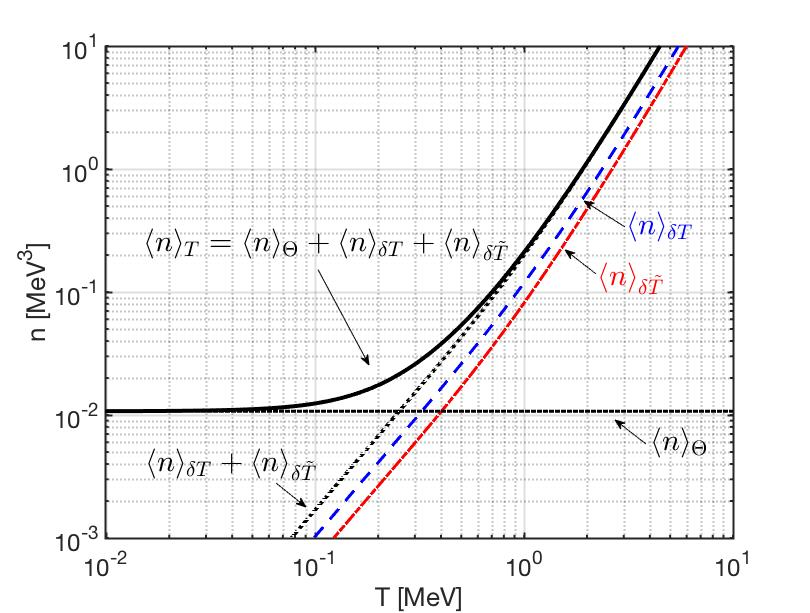
\includegraphics[width=0.5\textwidth]{./plot/Fermi_DenistyTest}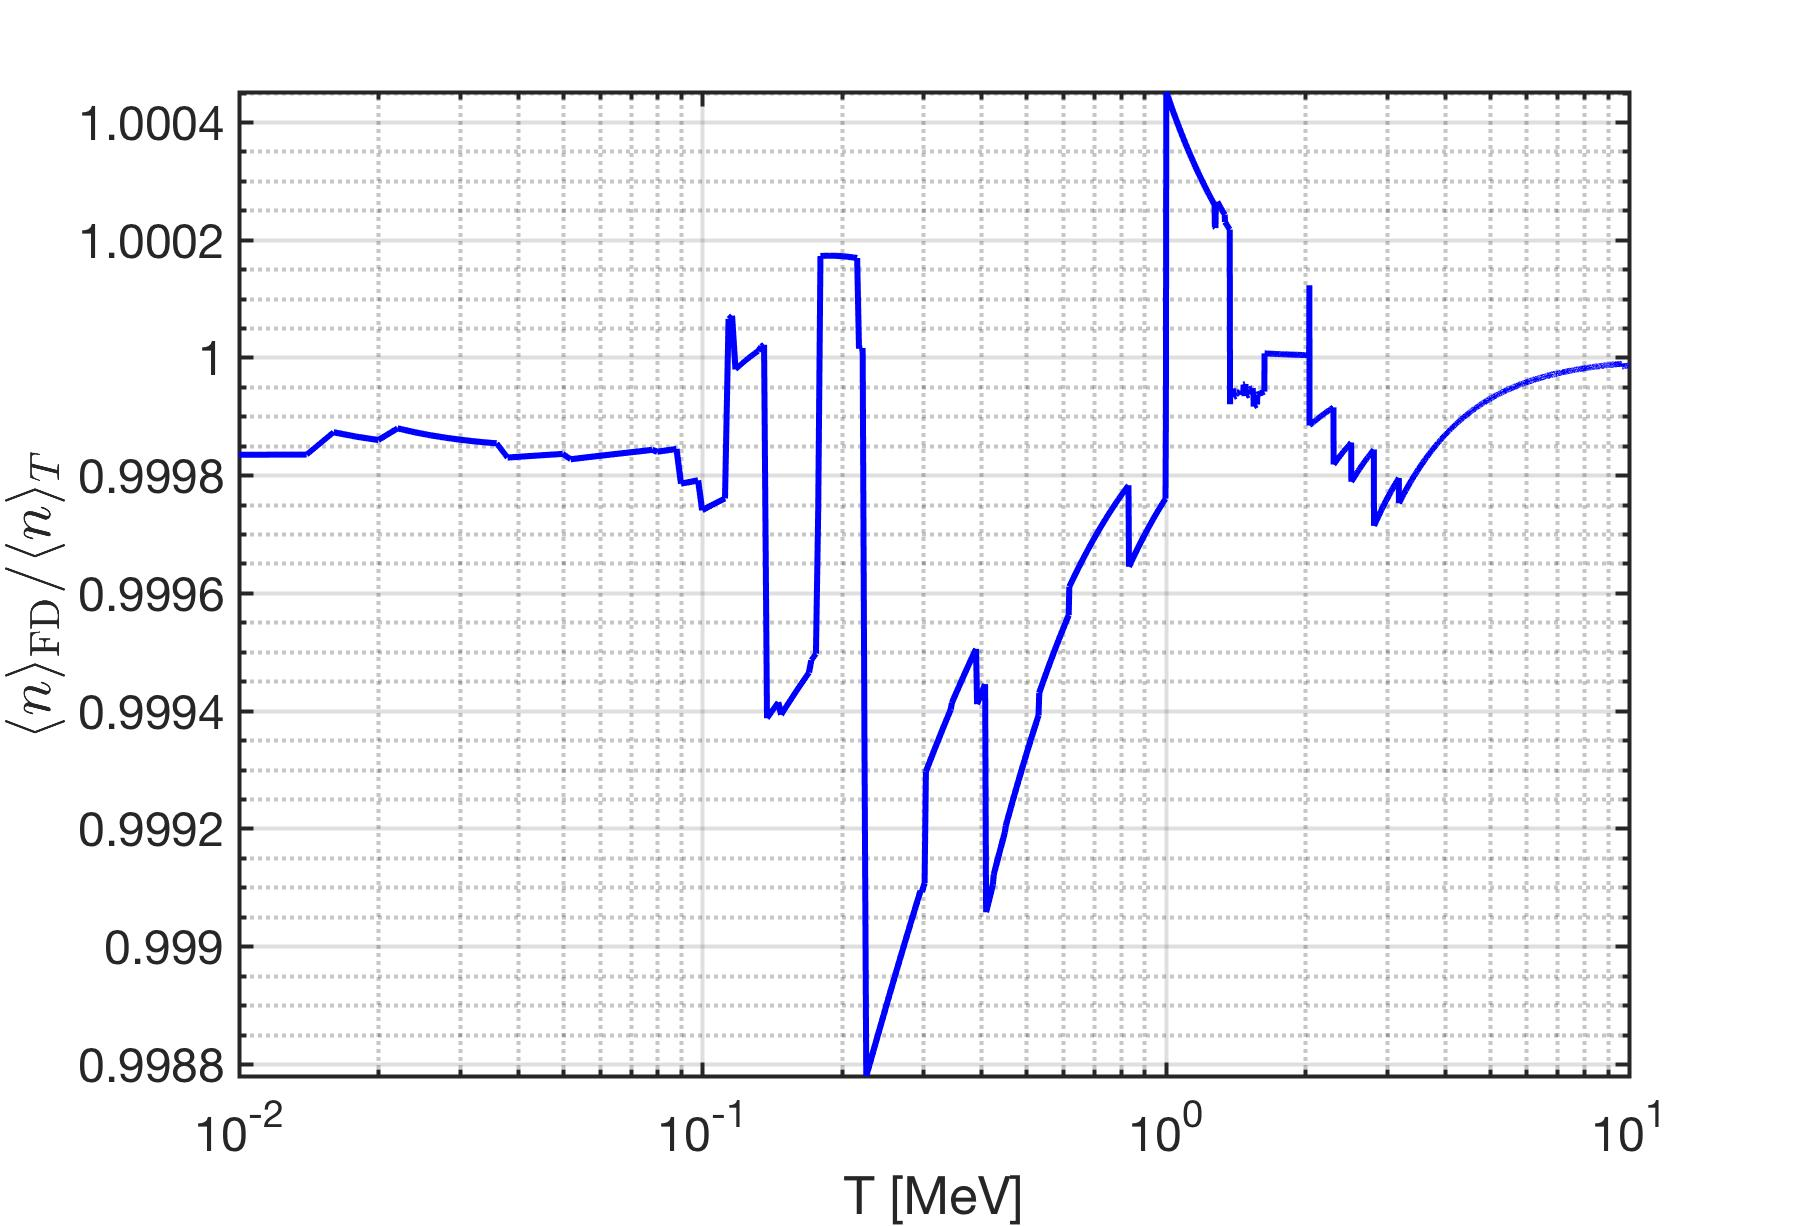
\includegraphics[width=0.55\textwidth]{./plot/FermiRatio5000}
\caption{(Left) The number density as a function of temperature by using  novel form of Fermi distribution Eq.~(\ref{DensitySum}). {\color{red}(Right) The density ratio between  Eq.~(\ref{DensityExact}) and Eq.~(\ref{DensitySum}), Still Working on this figure to make it better}. We consider $m=0.511$ MeV and $\tilde\mu=1$ MeV as an example.  }
\label{Density_checking}
\end{figure}
%%%%%%%%%%%%%%%%%%%%%%%%%%%%%%%%%%%%%%%




%By employing our decomposition form, we propose that the integral for finite temperature contribution $\langle G\rangle_{\delta T}$ in general can be written as
%\begin{align}\label{finite expansion}
%\langle G\rangle_{\delta T}=\sum_{n}c_nT^n,
%\end{align}
%where $c_n$ represents the coefficients used to expand the function in terms of temperature. In this scenario, our novel Fermi distribution can provide the tool to study any physical quantity when temperature approach to zero, and facilitate the connection between the study of finite temperature system to zero temperature limit smoothly. 

%In following we will demonstrate that for any general function in the zero-temperature limit, we can always write the integral into Eq.~(\ref{finite expansion}). 



%%%%%%%%%%%%%%%%%%%%%%%%%%%%%%%%%%%%%%%
\section{Results and Discussion}
\label{sec12}
In this work, we introduce a novel form of the Fermi distribution Eq.~(\ref{NFF1}) that separates the Fermi gas into zero and finite temperature components analytically. This is the first time in literature that has clean separation of the zero and finite temperature components. Unlike the traditional brutal approach to eliminating the $T=0$ limit from the low-temperature Fermi distribution, our novel form of the Fermi distribution for finite temperature component has several numerical advantages in computation. {\xgreen The prescription proposed here is in terms of distribution rather than analytical function. However, for all physical applications it is only necessary to calculate integrals for which the exact behavior at $x=0$ is not required.}

 
The mathematical form of the finite temperature components is well-suited for numerical calculations and can be used to address the integrals common in statistical physics. This is because the finite temperature components are naturally exponentially suppressed while also preserving the sign of all corrections making the formulation easier to numerically integrate and reduce the numerical noise, see Fig.~\ref{Fermi_Component}. We consider a semi relativistic-electron density where with high chemical potential $\mu>m$ at low temperature as an example. Fig.~\ref{Density_checking} shows the equivalence of particle number density with exact Fermi distribution Eq.~(\ref{DensityExact}) and our novel form  distribution Eq.~(\ref{DensitySum}). 
 
The Fermi distribution Eq.~(\ref{NFF1}) provides us the tool to study or examine the effects and characteristics of finite temperature components separately. In addition, our approach also allows for analytical exploration of the finite temperature contributions by expanding the function around the Fermi-energy surface.



%%%%%%%%%%%%%%%%%%%%%%%%%%%%%%%%%%%%%%%


% Martin - Highlight the method can be used to address the integrals common in stastistical physics.
% Johann - First time we separate cleanly the hot and cold components. This therefore could be very useful for studying interacting systems where the mathematics becomes intractible quickly. The properties near to the Fermi surface are clearly isolated and most of the interactions occur near the Fermi surface.
% Cold matter cannot form pairs, but finite temperature systems can because of the deformation of the step function. Particle-antiparticle hope pairs behavior is isolated. May have applications to superconducting systems. Allowing for the exploration of interacting systems at the Fermi surface.
% Reference to superconducting neutron stars.
% Andrew - This allows us to analyze the finite temperature elements as a distinct model.
% Cheng Tao - This novel form is numerically friendly as the finite temperature components are naturally exponentially suppresses while also preserving the sign of all corrections making the formulation easier to numerically integrate.

%%%%%%%%%%%%%%%%%%%%%%%%%%%%%%%%%%%%%%%
%\section{Appendix}
%\label{Append}
%%%%%%%%%%%%%%%%%%%%%%%%%%%%%%%%%%%%%%%
%%%%%%%%%%%%%%%%%%%%%%%%%%%%%%%%%%%%%%%%%%%
%%%%%%%%%%%%%%%%%%%%%%%%%%%%%%%%%%%%%%%
\backmatter

\bmhead{Acknowledgments}
We thank Gordon Baym and John W. Clark for their encouragement to publish this result.

%%%%%%%%%%%%%%%%%%%%%%%%%%%%%%%%%%%%%%%
\bibliography{novel-fermi-function-refs}
%% if required, the content of .bbl file can be included here once bbl is generated
%%\input sn-article.bbl
\end{document}
